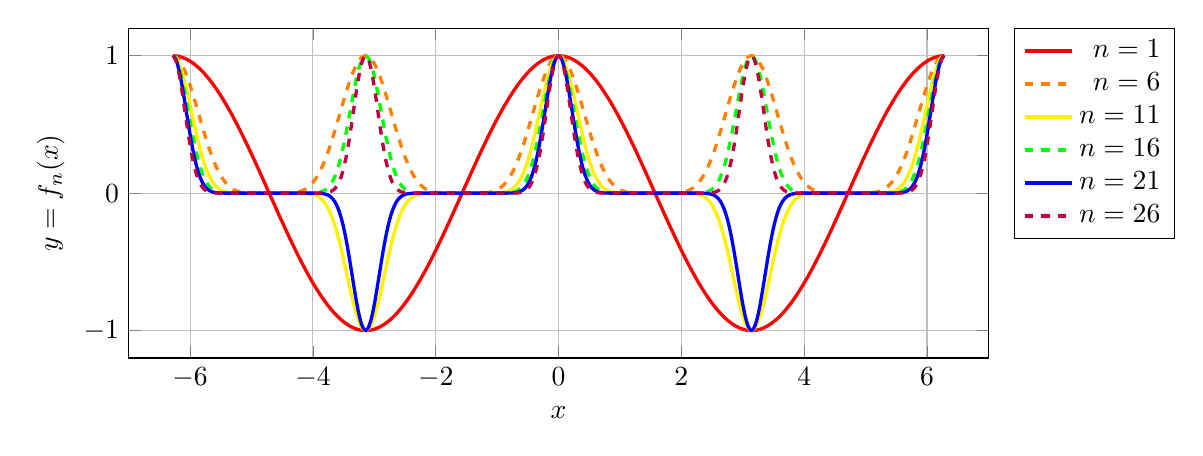
\begin{tikzpicture}[scale=1]
    \begin{axis}[
        xlabel=$x$,
        ylabel={$y=f_{n}(x)$},
        width=12.5cm,
        height=5.77cm,
        grid=major,
        xmin=-7, xmax=7,
        ymin=-1.2, ymax=1.2,
        legend style={
            cells={anchor=east},
            legend pos=outer north east,
        }
    ]
        \addplot[color=red, samples=500, domain=-2*pi:2*pi, very thick] {cos(deg(x))^1};
        \addlegendentry{$n=1$}
        \addplot[color=orange, samples=500, domain=-2*pi:2*pi, very thick, dashed] {cos(deg(x))^6};
        \addlegendentry{$n=6$}
        \addplot[color=yellow, samples=500, domain=-2*pi:2*pi, very thick] {cos(deg(x))^11};
        \addlegendentry{$n=11$}
        \addplot[color=green, samples=500, domain=-2*pi:2*pi, very thick, dashed] {cos(deg(x))^16};
        \addlegendentry{$n=16$}
        \addplot[color=blue, samples=500, domain=-2*pi:2*pi, very thick] {cos(deg(x))^21};
        \addlegendentry{$n=21$}
        \addplot[color=purple, samples=500, domain=-2*pi:2*pi, very thick, dashed] {cos(deg(x))^26};
        \addlegendentry{$n=26$}
    \end{axis}
\end{tikzpicture}